%Version 3.1 December 2024
% Springer Nature LaTeX Template for Neural Computing and Applications (NCA)
% Single-column layout using sn-jnl class

\documentclass[pdflatex,sn-mathphys-num]{sn-jnl}

%%%% Standard Packages
\usepackage{graphicx}%
\usepackage{multirow}%
\usepackage{tabularx}%
\usepackage{amsmath,amssymb,amsfonts}%
\usepackage{amsthm}%
\usepackage{mathrsfs}%
\usepackage{textcomp}%
\usepackage{booktabs}%
\usepackage{float}%
\usepackage{subcaption}%
\usepackage{hyperref}%
\raggedbottom

\begin{document}

\title[PinPoint: Interpretable Multimodal Deepfake Detection]{PinPoint: An Interpretable Multimodal Architecture for Deepfake Detection with Comprehensive Explainable AI Analysis}

%%=============================================================%%
%% ORCID IDs: Please add your 16-digit ORCID IDs below
%%=============================================================%%

\author[1]{\fnm{Palak} \sur{Parmar} \orcid{0009-0000-2114-7114}}\email{24rcp002@sot.pdpu.ac.in}


\author*[2]{\fnm{Chintan} \sur{Bhatt} \orcid{0000-0002-0423-0159}}\email{cbhatt@uow.edu.au}

\author[1]{\fnm{SantoshKumar} \sur{Bharti} \orcid{0000-0002-0627-6433}}\email{santosh.bharti@sot.pdpu.ac.in}


\affil*[1]{\orgdiv{Department of Computer Science and Engineering, School of Science and Technology}, \orgname{Pandit Deendayal Energy University}, \orgaddress{\city{Gandhinagar}, \state{Gujarat}, \country{India}}}

\affil[2]{\orgname{University of Wollongong}, \orgaddress{\country{Australia}}}

\abstract{Manipulated audiovisual media creates a growing challenge for digital forensics because detectors must be both accurate and auditable. Many deepfake detectors still rely on generator-specific visual or spectral artifacts, and their explanations often remain post-hoc visualizations that do not verify whether the model used meaningful forensic evidence. This paper presents PinPoint, an interpretable audio--visual deepfake detector that makes temporal synchrony an explicit learning objective. PinPoint combines an XAI-compatible ResNet-18 visual encoder, a CNN--GRU audio encoder, stacked gated cross-attention blocks, a three-stage curriculum, and a synchronization loss that encourages diagonal, smooth, high-energy attention maps for aligned real samples. On a unified LAV-DF and FakeAVCeleb benchmark, PinPoint achieves 97.47\% accuracy over 26,097 test samples, with 0.968 macro F1 and 0.9825 F1 for the fake class. Ablations show that removing the synchronization loss, gated fusion, or curriculum reduces accuracy to 75.47\%, 58.35\%, and 81.44\%, respectively. A multimodal Explainable Artificial Intelligence (XAI) suite combining Integrated Gradients, Layer-wise Relevance Propagation, SHapley Additive exPlanations, attention analysis, counterfactuals, and Testing with Concept Activation Vectors links these decisions to lip-sync and audio--visual mismatch cues. The results indicate that synchrony-aware supervision can improve both detection performance and the auditability of model explanations.}

\keywords{Deepfake Detection, Multimodal Learning, Explainable AI, Temporal Synchronization, Curriculum Learning}

\maketitle

\section{Introduction}\label{sec1}

Generative models can now produce manipulated speech and facial motion with enough realism to affect journalism, legal evidence, political communication, and personal reputation. This progress makes deepfake detection a forensic problem rather than only a classification benchmark: a useful detector must identify manipulated content accurately and provide evidence that an examiner can inspect. Recent surveys emphasize that audio--visual deepfake detection remains difficult because manipulations vary across generators, compression settings, languages, and recording conditions \cite{ref13,ref22}.

Early detectors often focused on unimodal artifacts such as facial texture defects, color inconsistency, blending traces, or spectral irregularities. These cues can be effective when test samples resemble the training distribution, but they are fragile when a detector faces unseen generation pipelines or post-processing transformations \cite{ref3,ref16}. Audio-only approaches face the same limitation: a model can learn synthesis artifacts that disappear as voice generation improves. Robust forensic detection therefore needs cues that are harder for a generator to hide. One such cue is temporal consistency between what is spoken and what the face does while speaking.

\begin{figure}[H]
\centering
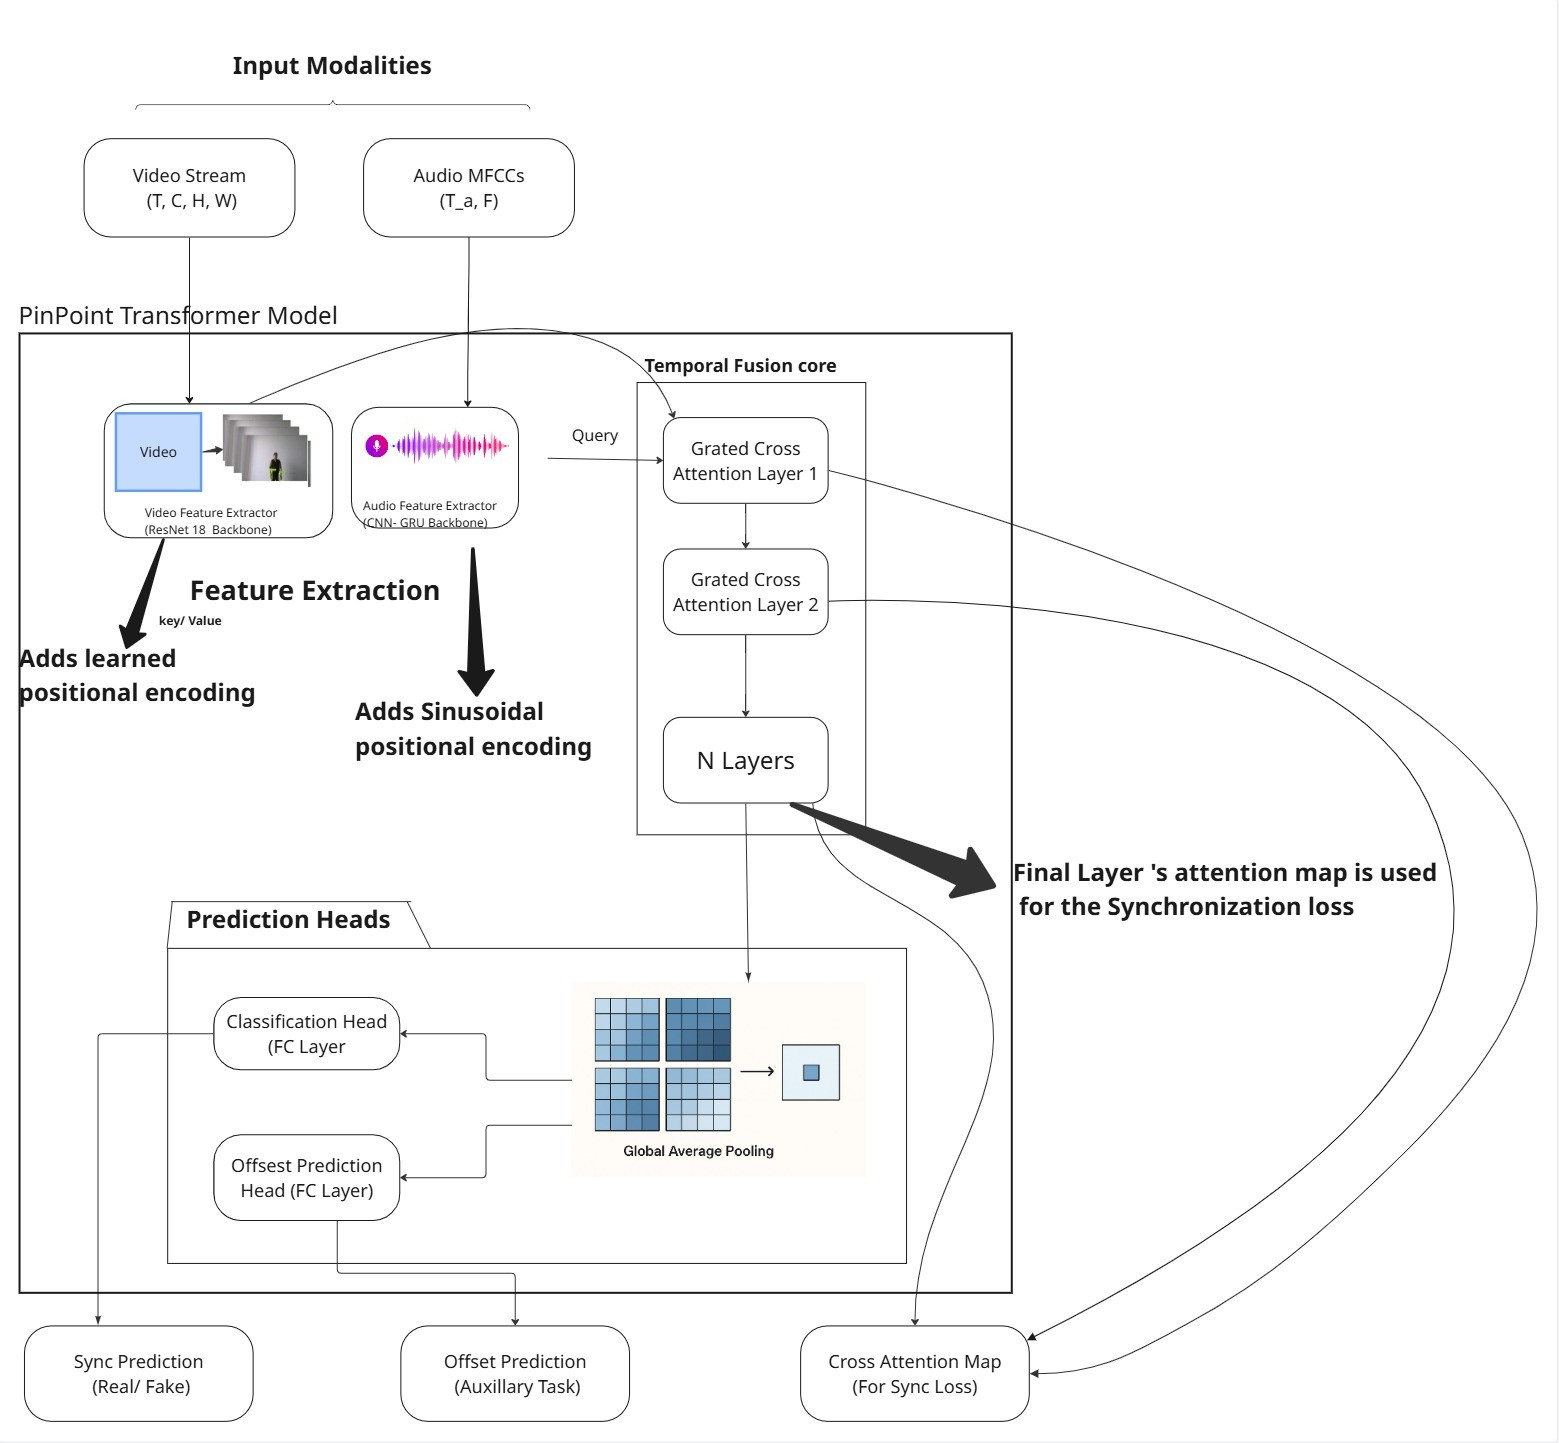
\includegraphics[width=0.8\textwidth]{images/image1.jpeg}
\caption{The PinPoint Architecture and Training Framework. This multi-panel figure provides a complete overview. (a) The core architecture shows the flow from Video/Audio inputs to classification. (b) The curriculum learning timeline illustrates the three training phases. (c) A conceptual diagram explains the goal of the synchronization loss.}\label{fig1}
\end{figure}

Multimodal detectors address this issue by jointly processing the acoustic and visual streams, but fusion alone does not guarantee synchrony-aware reasoning. Cross-attention models can still learn shortcut correlations if the training objective rewards only the final real/fake decision. In high-stakes settings, this is not sufficient. A forensic detector should expose whether it relied on lip motion, acoustic timing, mouth-region evidence, or unrelated artifacts, and these explanations should be evaluated quantitatively rather than only displayed as heatmaps \cite{ref4,ref8,ref17}.

We introduce PinPoint, a synchronization-aware and explanation-oriented framework for audio--visual deepfake detection. Figure~\ref{fig1} summarizes the model, curriculum, and synchronization loss. PinPoint uses a ResNet-18 video encoder, a CNN--GRU audio encoder, and stacked gated cross-attention blocks that allow audio features to attend to temporally corresponding visual features. During training, a multi-component synchronization loss constrains attention maps for aligned real samples to remain diagonal, dominant near the diagonal, and temporally smooth. A three-stage curriculum first stresses audio reliance, then synchronization, and finally full multimodal fusion.

Our contributions are as follows:
\begin{enumerate}
\item We propose a gated cross-attention architecture for audio--visual deepfake detection that explicitly models speech-face temporal correspondence rather than treating multimodal fusion as a generic feature-combination step.
\item We introduce a synchronization loss that shapes cross-attention maps into interpretable temporal structures and use it together with an auxiliary offset-prediction task.
\item We train the detector with a three-stage curriculum designed to reduce shortcut learning and improve robustness to missing or weak modality evidence.
\item We evaluate model reasoning with a multimodal XAI suite, including local attribution, attention analysis, counterfactuals, and concept activation analysis, and report quantitative explanation metrics alongside classification metrics.
\item We validate the design through full-model and ablation experiments on a unified LAV-DF and FakeAVCeleb benchmark, where the complete model achieves 97.47\% accuracy and each removed component causes a clear performance drop.
\end{enumerate}

The remainder of the paper reviews related work, presents the PinPoint architecture and training objectives, describes the XAI framework, reports quantitative and qualitative results, and discusses limitations for deployment-oriented forensic use.


\section{Related Work}\label{sec2}

This section reviews three lines of work that shape PinPoint: deepfake detector architectures, explainability for multimedia forensics, and training strategies for generalization. Table~\ref{tab:comparison} summarizes representative methods and the gap each leaves for synchronization-aware explanation.


\subsection{Architectural Evolution in Deepfake Detection}\label{sec2.1}

Visual deepfake detectors have traditionally relied on spatial artifacts in faces, including blending boundaries, texture irregularities, color mismatch, and manipulation-specific noise. These approaches remain useful baselines, especially when paired with contrastive learning or strong augmentation \cite{ref3}. Their central limitation is that they often learn the artifacts of known generators rather than the physical and semantic constraints of authentic audiovisual communication. As generation pipelines improve, surface artifacts become weaker and less reliable.

Multimodal methods attempt to overcome this limitation by combining speech and facial evidence. Multimodaltrace uses audiovisual representation learning to fuse modality-specific features \cite{ref1}, while temporal feature prediction and synchronization-focused methods model alignment between audio and video streams \cite{ref2,ref5}. More recent approaches use cross-modal alignment, distillation, or hierarchical pre-training to strengthen shared representations \cite{ref7,ref11,ref12}. These methods show that audio--visual information improves detection, but many still optimize the final classification objective without directly constraining the structure of cross-modal attention. PinPoint addresses this gap by treating synchronization as a supervised property of the learned attention map.


\subsection{Explainable AI in Multimedia Forensics}\label{sec2.2}

Interpretability is essential in multimedia forensics because a correct prediction is not enough when the decision may support an investigation. Visual interpretability methods such as Grad-CAM can show where a model looks, but spatial saliency alone does not prove that the detector used a meaningful manipulation cue \cite{ref21}. Prototype-based detectors improve transparency by linking decisions to representative learned features \cite{ref18,ref24}, and recent multimodal systems generate explanations intended for non-expert users \cite{ref9,ref14}. These approaches make detector behavior easier to inspect, but their explanations are often qualitative and may not measure stability, sparsity, or agreement across explanation methods.
Quantitative XAI studies have begun to evaluate explanations using metrics such as focus, consistency, robustness, and attribution agreement \cite{ref4,ref8}. This direction is important for deepfake detection because forensic users need to know whether explanations are repeatable and whether different attribution methods identify similar evidence. PinPoint builds on this line of work by evaluating not only video saliency, but also audio attribution, attention structure, counterfactual sensitivity, and concept-level response to lip-sync error.

\subsection{Learning Strategies for Robust Multimodal Detection}\label{sec2.3}


Generalization remains difficult because deepfake datasets differ in manipulation type, compression level, language, speaker identity, and recording conditions. Contrastive objectives, explicit correlation learning, and temporal modeling can reduce shortcut learning by pushing models toward more stable features \cite{ref3,ref10,ref11}. However, a model can still over-rely on the easiest available modality if both streams are presented normally throughout training.

Curriculum learning offers a way to control which evidence the model learns first. Instead of presenting the full multimodal task from the beginning, PinPoint uses a staged procedure: heavy video masking first encourages audio reliance, synchronization-focused training then strengthens temporal alignment, and full multimodal training finally combines all evidence. This design is intended to make cross-modal synchrony a learned decision cue rather than an incidental by-product of feature fusion.

\begin{table}[htbp]
\caption{Comparative Analysis of Deepfake Detection Approaches}\label{tab:comparison}
\scriptsize
\setlength{\tabcolsep}{3pt}
\begin{tabularx}{\textwidth}{@{}p{2.2cm}p{0.9cm}p{2.9cm}p{2.1cm}X@{}}
\toprule
\textbf{Method} & \textbf{Modality} & \textbf{Core Technique} & \textbf{Interpretability} & \textbf{Remarks} \\
\midrule
XceptionNet \cite{ref3} & Visual & CNN-based artifact detection & Grad-CAM & Strong visual baseline; limited cross-generator generalization \\
Multimodaltrace \cite{ref1} & A--V & MLP-Mixer fusion & Post-hoc saliency maps & Joint multimodal fusion; no explicit temporal modeling \\
AVSFF \cite{ref5} & A--V & TCN-BiLSTM + DTW & Minimal & Explicit alignment modeling; high computation \\
CAD \cite{ref7} & A--V & Cross-attention with CLIP/Whisper & Attention visualization & Semantic cross-modal alignment; lacks sync-aware loss \\
ConvNext-PNet \cite{ref18} & Visual & Prototype learning & Inherent interpretability & Clear decision pathways; visual-only limitation \\
ExDDV \cite{ref9} & A--V & MLLM-based explanations & Language-based reasoning & Improved user understanding; lacking quant.\ validation \\
HOLA \cite{ref12} & A--V & Hierarchical pre-training & None & Strong multimodal representation; opaque reasoning \\
PinPoint (Ours) & A--V & Gated cross-attn.\ + sync.\ loss & Multi-method XAI & Interpretable sync-aware detection; slightly higher compute cost \\
\botrule
\end{tabularx}
\end{table}


\section{Proposed Method: PinPoint Architecture}\label{sec3}

PinPoint is designed to make audio--visual synchrony both useful for classification and visible during explanation. The framework combines modality-specific encoders, gated cross-attention fusion, curriculum learning, and a multi-component synchronization loss that directly supervises the temporal structure of the attention map.

\begin{figure}[H]
\centering
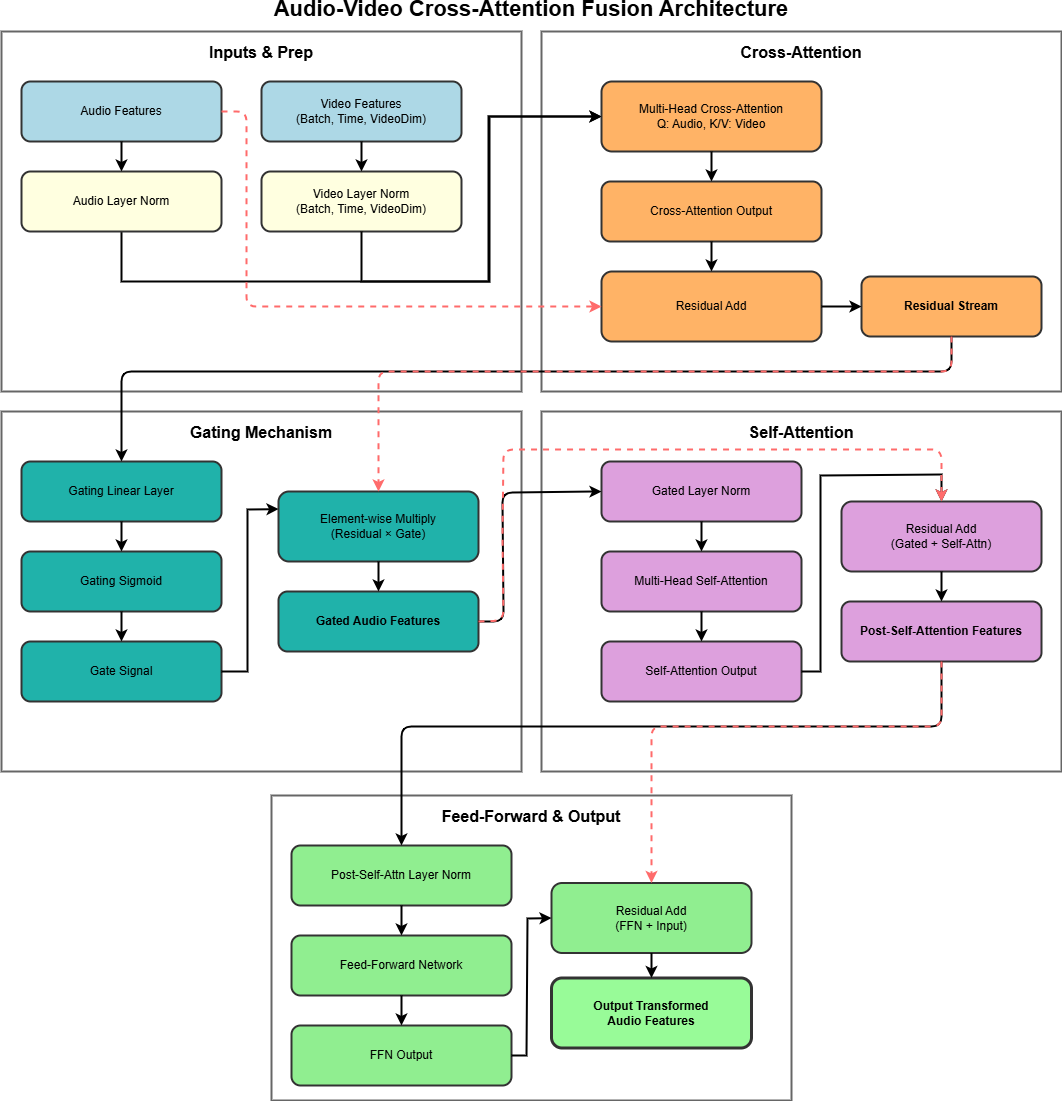
\includegraphics[width=0.7\textwidth]{images/image2.png}
\caption{Gated cross-attention block. Audio features act as the query and video features act as keys and values. The attended audio representation then passes through a learned gate, self-attention, and a feed-forward network before classification.}\label{fig2}
\end{figure}


\subsection{Overall Framework}\label{sec3.1}

PinPoint receives 30 normalized video frames of size $128 \times 128$ and a time sequence of 13-dimensional Mel-frequency cepstral coefficient (MFCC) features. The video stream is encoded with an ImageNet-pretrained ResNet-18. We remove in-place operations from the residual blocks so that gradient-based XAI methods can backpropagate through the network reliably. The final convolutional features are adaptively pooled and projected to a 256-dimensional embedding.

The audio stream uses two one-dimensional convolution layers followed by layer normalization and a Gated Recurrent Unit (GRU). The convolution layers capture local acoustic patterns, while the GRU preserves longer temporal dependencies in the MFCC sequence. Video embeddings receive a learned positional encoding; audio embeddings receive sinusoidal positional encodings.

Fusion is performed by three gated cross-attention blocks. In each block, the audio sequence queries the video sequence, so the attention map describes which video frames support each audio timestep. The attended representation is filtered by a sigmoid gate, passed through audio self-attention and a feed-forward network, and finally mean-pooled over audio time. PinPoint uses two output heads: a binary classification head for real/fake prediction and an auxiliary offset head with $2M+1$ classes, where $M=5$ is the maximum frame offset used during synchronization training.


\subsection{Curriculum Learning Pipeline}\label{sec3.2}

The curriculum controls which evidence the model can use during different parts of training. This prevents the network from immediately exploiting the easiest visual shortcut and gives the synchronization objective a dedicated learning phase.

\textbf{Phase 1: Forced Audio Reliance.} During the first two epochs, we randomly mask 50--80\% of video frames. This forces the network to learn useful audio features rather than depending only on visual artifacts.

\textbf{Phase 2: Synchronization Focus.} During the next three epochs, the model emphasizes synchronized real samples and learns the desired diagonal attention structure. The auxiliary offset loss is down-weighted in this phase so that the synchronization loss dominates the alignment signal.

\textbf{Phase 3: Holistic Fusion.} For the remaining epochs, the full multimodal input and complete composite loss are used. This final phase lets the model combine visual, acoustic, and synchronization evidence.

The ablation study in Section~\ref{sec5.2} shows that removing this curriculum reduces full-test accuracy from 97.47\% to 81.44\%, indicating that staged optimization is important for the final detector. The synchronization loss that guides Phase 2 of this curriculum is formalized as follows.


\subsection{Advanced Synchronization Loss}\label{sec3.3}

The synchronization loss shapes the final cross-attention map into an interpretable structure for real samples whose audio and video are aligned. Let $\mathbf{A}\in\mathbb{R}^{N\times M}$ denote the attention map between $N$ audio timesteps and $M$ video frames. The loss combines direct target matching, diagonal dominance, and temporal smoothness:

\begin{equation}\label{eq1}
\mathcal{L}_{\text{sync}} = \lambda_1 \mathcal{L}_{\text{MSE}} + \lambda_2 \mathcal{L}_{\text{diag}} + \lambda_3 \mathcal{L}_{\text{smooth}}
\end{equation}

where $\lambda_1=1.0$, $\lambda_2=0.5$, and $\lambda_3=0.2$ in our implementation.

\textbf{1. Direct target matching.} The first term computes mean-squared error between $\mathbf{A}$ and a soft diagonal target $\mathbf{T}$:

\begin{equation}\label{eq2}
\mathcal{L}_{\text{MSE}} = \frac{1}{N \times M} \sum_{i=1}^{N} \sum_{j=1}^{M} (A_{ij} - T_{ij})^2
\end{equation}

The target maps each audio timestep $i$ to a corresponding video-frame center $c_i=\lfloor i/r\rfloor$, where $r=2$ MFCC timesteps per video frame. It then normalizes a Gaussian band over video positions:

\begin{equation}\label{eq3}
T_{ij} = \frac{\exp\!\left(-\frac{(j-c_i)^2}{2\sigma^2}\right)}
{\sum_{m=1}^{M}\exp\!\left(-\frac{(m-c_i)^2}{2\sigma^2}\right)}
\end{equation}

\textbf{2. Diagonal dominance.} The second term penalizes attention energy outside a bandwidth $b$ around the synchronized audio--video correspondence:

\begin{equation}\label{eq4}
\mathcal{L}_{\text{diag}} = 1 - \frac{\displaystyle\sum_{i=1}^{N}\sum_{|j-c_i| \le b} A_{ij}}{\displaystyle\sum_{i=1}^{N}\sum_{j=1}^{M} A_{ij}}
\end{equation}

We use $b=2$, matching the implementation's synchronization bandwidth.

\textbf{3. Temporal smoothness.} The third term discourages abrupt attention changes across adjacent audio and video positions:

\begin{equation}\label{eq5}
\mathcal{L}_{\text{smooth}} = \frac{1}{N-1} \sum_{i=1}^{N-1} \sum_{j=1}^{M} (A_{i,j} - A_{i+1,j})^2 + \frac{1}{M-1} \sum_{i=1}^{N} \sum_{j=1}^{M-1} (A_{i,j} - A_{i,j+1})^2
\end{equation}

This objective makes the learned attention map part of the model design rather than only a post-hoc visualization. For a synchronized real sample, a diagonal map indicates that speech acoustics and facial motion support each other; a diffuse or off-diagonal map indicates weaker temporal correspondence.


\subsection{Training Objectives}\label{sec3.4}

PinPoint is trained end-to-end with a weighted composite loss:

\begin{equation}\label{eq6}
\mathcal{L}_{\text{total}} = W_{\text{class}} \cdot \mathcal{L}_{\text{class}} + W_{\text{offset}} \cdot \mathcal{L}_{\text{offset}} + W_{\text{sync}} \cdot \mathcal{L}_{\text{sync}}
\end{equation}

$\mathcal{L}_{\text{class}}$ uses Binary Cross-Entropy with Logits, incorporating a $\text{pos\_weight}$ term to address class imbalance:

\begin{equation}\label{eq7}
\mathcal{L}_{\text{class}} = -\frac{1}{N} \sum_{i=1}^{N} \left[ w_i \, y_i \log(\hat{y}_i) + (1 - y_i) \log(1 - \hat{y}_i) \right]
\end{equation}

where $y_i$ is the ground truth, $\hat{y}_i$ is the predicted probability, and $w_i$ is the class-imbalance weight. $\mathcal{L}_{\text{offset}}$ is standard cross-entropy for auxiliary offset prediction on real samples:

\begin{equation}\label{eq8}
\mathcal{L}_{\text{offset}} = -\sum_{k=1}^{K} y_k \log(\hat{y}_k)
\end{equation}

where $K=11$ is the number of offset classes and $y_k$ is the one-hot offset label. $\mathcal{L}_{\text{sync}}$ applies only to real samples with zero artificial offset. Table~\ref{tab:hyper} lists the main implementation settings.

\begin{table}[htbp]
\caption{Key Hyperparameters for PinPoint Training}\label{tab:hyper}
\begin{tabular}{@{}ll@{}}
\toprule
\textbf{Parameter} & \textbf{Value} \\
\midrule
\multicolumn{2}{@{}l@{}}{\textit{Loss Weights}} \\
\quad $W_{\text{class}}$ & 1.0 \\
\quad $W_{\text{offset}}$ & 0.5 \\
\quad $W_{\text{sync}}$ & 3.0 \\
\midrule
\multicolumn{2}{@{}l@{}}{\textit{Sync Loss Components}} \\
\quad $\lambda_1$ (MSE weight) & 1.0 \\
\quad $\lambda_2$ (Diagonal weight) & 0.5 \\
\quad $\lambda_3$ (Smoothness weight) & 0.2 \\
\quad $\sigma$ (Gaussian width) & 2.0 \\
\quad $b$ (Diagonal bandwidth) & 2 \\
\midrule
\multicolumn{2}{@{}l@{}}{\textit{Model and Training}} \\
\quad Video input & 30 frames, $128 \times 128$ \\
\quad Audio input & 13 MFCC coefficients \\
\quad Embedding dimension & 256 \\
\quad Attention heads / layers & 8 / 3 \\
\quad Dropout & 0.1 \\
\quad Batch size / epochs & 4 / 15 \\
\quad Learning rate & $1 \times 10^{-4}$ \\
\quad Weight decay & $1 \times 10^{-4}$ \\
\quad Optimizer & AdamW \\
\quad Scheduler & Cosine Annealing \\
\quad Modality dropout & 0.15 \\
\botrule
\end{tabular}
\end{table}


\section{Comprehensive Explainable AI Framework}\label{sec4}

PinPoint includes an XAI pipeline because the detector is intended for forensic inspection, not only benchmark scoring. The pipeline combines feature attribution, attention analysis, counterfactual testing, and concept sensitivity so that model behavior can be examined at the pixel, acoustic-feature, temporal-alignment, and semantic-concept levels.


\subsection{XAI Techniques Employed}\label{sec4.1}

Our framework systematically analyzes model behavior at multiple levels, spanning from local attribution to concept sensitivity.

\textbf{Local attribution methods.} Integrated Gradients estimates feature importance by accumulating gradients along a path from a baseline input to the observed sample. Layer-wise Relevance Propagation backpropagates relevance scores through the network, while SHapley Additive exPlanations (SHAP) estimate feature contribution relative to background samples. We apply these methods to both video frames and MFCC features so that visual and acoustic evidence can be inspected together.

\textbf{Attention-based explanations.} Because PinPoint uses audio-to-video cross-attention, attention maps have a direct temporal interpretation: diagonal structure indicates that audio timesteps attend to corresponding video frames. We also use attention rollout and attention-flow visualizations to inspect how evidence moves through stacked gated cross-attention layers.

\textbf{Counterfactual explanations.} Counterfactual analysis searches for small video and audio perturbations that change the predicted class. These perturbations provide a causal stress test: if changing mouth-region texture or synchronization-related acoustic cues flips the prediction, the explanation is stronger than a static saliency map alone.

\textbf{Concept activation analysis.} Testing with Concept Activation Vectors (TCAV) trains linear concept classifiers on internal activations and measures whether moving in a human-defined concept direction changes the model's output \cite{ref8}. We use this analysis to test sensitivity to the lip-sync error concept.

\subsection{Unified Visualization and Quantitative Metrics}\label{sec4.2}

The visualization module combines all explanations for a single sample (Figure~\ref{fig3}). It overlays visual saliency on frames, plots MFCC attribution over time, displays attention maps, and records the predicted class and confidence.

We report three quantitative explanation metrics inspired by prior XAI evaluation work \cite{ref4,ref8}:

\textbf{Focus and sparsity (Gini index).} The Gini index measures how concentrated an attribution map is. Higher values indicate sparse evidence concentrated in fewer regions or timesteps; lower values indicate more diffuse attribution.

\begin{equation}\label{eq9}
G = \frac{\displaystyle\sum_{i=1}^{n} (2i - n - 1) x_i}{\displaystyle n\sum_{i=1}^{n} x_i}
\end{equation}

where $x_i$ are sorted attribution values and $n$ is the number of features. $G=1$ indicates maximal concentration on one feature, while $G=0$ indicates a uniform attribution distribution.

\textbf{Feature agreement.} Feature agreement measures whether explanations for different fake samples highlight similar regions. We compute it by normalizing the variance across attribution maps:

\begin{equation}\label{eq10}
\text{Agreement} = 1 - \frac{\text{Var}(A_1, A_2, \ldots, A_N)}{\text{max possible variance}}
\end{equation}

where $A_i$ is the attribution map for sample $i$.

\textbf{Inter-technique consistency.} This metric computes Spearman's rank correlation between attribution maps from different explanation methods, such as Integrated Gradients and Layer-wise Relevance Propagation:

\begin{equation}\label{eq11}
\rho = 1 - \frac{6 \sum d_i^2}{n(n^2 - 1)}
\end{equation}

where $d_i$ is the rank difference for feature $i$. A higher correlation indicates that multiple explanation methods identify similar forensic cues.

\begin{figure}[H]
\centering
\begin{subfigure}[b]{0.32\textwidth}
\centering
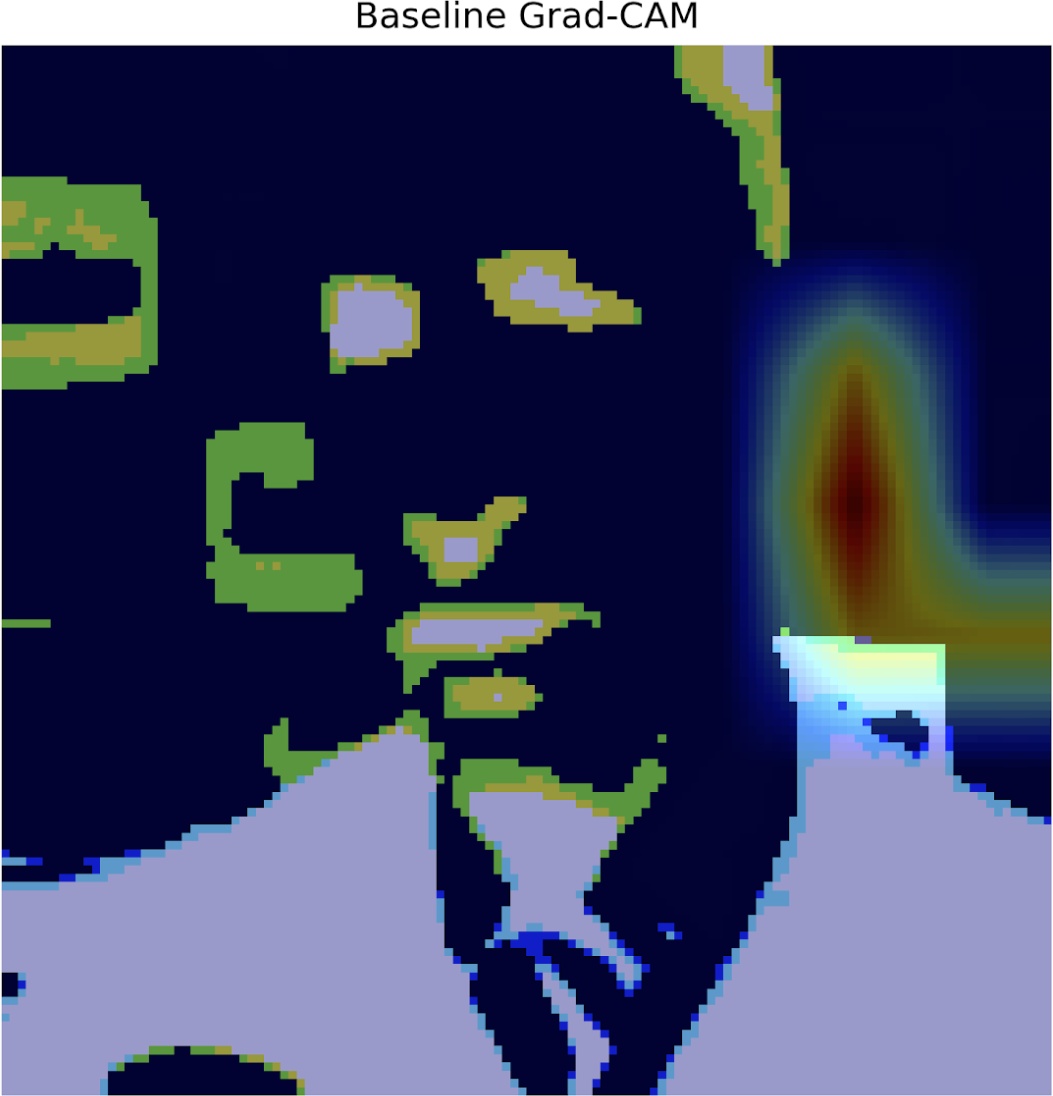
\includegraphics[width=\textwidth]{images/image3.png}
\caption{Baseline Grad-CAM}
\end{subfigure}\hfill
\begin{subfigure}[b]{0.32\textwidth}
\centering
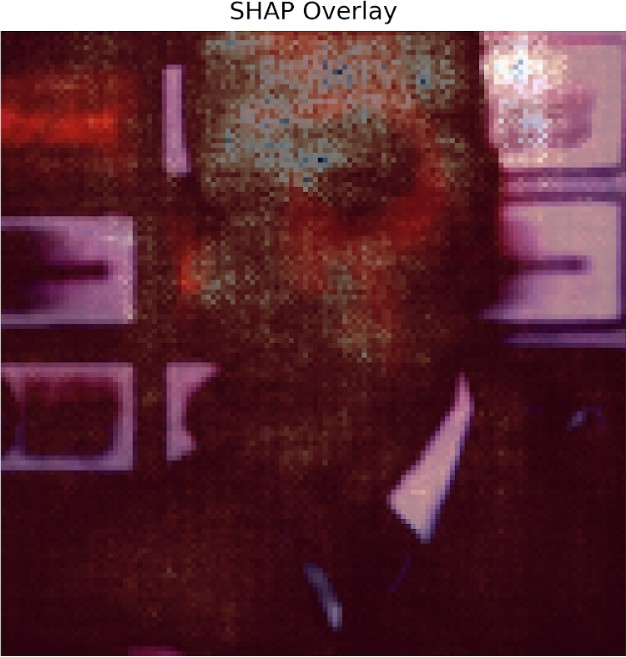
\includegraphics[width=\textwidth]{images/image4.jpeg}
\caption{SHAP Overlay}
\end{subfigure}\hfill
\begin{subfigure}[b]{0.32\textwidth}
\centering
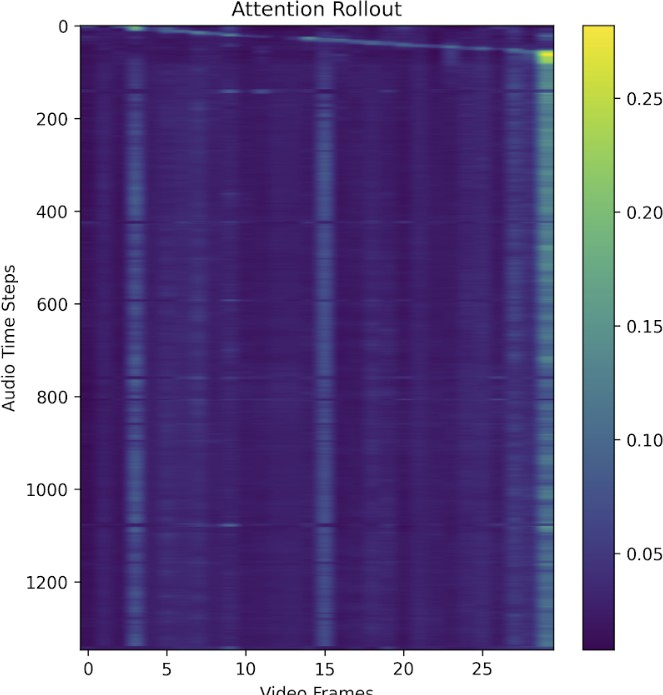
\includegraphics[width=\textwidth]{images/image5.jpeg}
\caption{Attention Rollout}
\end{subfigure}
\caption{Multimodal XAI suite for a fake sample: (a) Grad-CAM highlights mouth-region evidence, (b) SHAP shows frame-level attribution, and (c) attention rollout visualizes weak diagonal audio--visual alignment.}\label{fig3}
\end{figure}


\section{Experiments, Results, and Analysis}\label{sec5}


\subsection{Experimental Setup}\label{sec5.1}


\subsubsection{Dataset Description}\label{sec5.1.1}

\textbf{LAV-DF Dataset.} LAV-DF provides manipulated videos with audio--visual inconsistencies and supports evaluation of temporal mismatch cues.

\textbf{FakeAVCeleb Dataset.} FakeAVCeleb contains celebrity videos manipulated across audio and visual modalities, making it useful for testing multimodal detector behavior.

For the unified experiments, we use the standard identity-independent LAV-DF train/validation/test partition and evaluate on the locally available preprocessed test set. Table~\ref{tab:split} reports the split sizes and class balance used for training, validation, and testing.

\begin{table}[htbp]
\caption{Dataset Split Sizes and Class Balance}\label{tab:split}
\begin{tabular}{@{}lrrrr@{}}
\toprule
\textbf{Split} & \textbf{Total} & \textbf{Real} & \textbf{Fake} & \textbf{Real/Fake Ratio} \\
\midrule
Train & 78,703 & 21,254 & 57,449 & 0.37 \\
Validation & 31,501 & 8,271 & 23,230 & 0.36 \\
Test & 26,097 & 6,906 & 19,191 & 0.36 \\
\botrule
\end{tabular}
\end{table}


\subsubsection{Benchmark Construction}\label{sec5.1.2}

\begin{itemize}
\item Each sample uses 30 video frames resized to $128 \times 128$.
\item Audio is represented as 13-dimensional MFCC features.
\item The training split contains 78,703 samples: 21,254 real and 57,449 fake.
\item The validation split contains 31,501 samples: 8,271 real and 23,230 fake.
\item The unified test split contains 26,097 samples: 6,906 real and 19,191 fake.
\item We use the original identity-independent split and do not re-split the data; the inherited split is approximately class-stratified across train, validation, and test.
\item Training includes artificial audio offsets for real samples to supervise the auxiliary offset head.
\end{itemize}


\subsubsection{Implementation Details}\label{sec5.1.3}

We implement PinPoint in PyTorch and train with automatic mixed precision. The optimizer is AdamW with learning rate $1\times10^{-4}$, weight decay $1\times10^{-4}$, cosine annealing, batch size 4, and 15 epochs. Training augmentations include JPEG compression, random noise, Gaussian blur, resizing artifacts, color jitter, random erasing, modality dropout, and curriculum video masking. Table~\ref{tab:hyper} reports the main settings.


\subsection{Quantitative Performance and Ablation Studies}\label{sec5.2}

\textbf{Main performance.} Table~\ref{tab3} reports the full PinPoint model on the unified test split. The model achieves 97.47\% accuracy over 26,097 samples, with macro F1 of 0.968. Performance is strongest on the fake class, where the model reaches 0.9825 F1, while real-class recall remains high at 0.98.

\begin{table}[htbp]
\caption{Performance Metrics of Full PinPoint Model on Unified Test Set}\label{tab3}
\begin{tabular}{@{}lcccc@{}}
\toprule
\textbf{Class} & \textbf{Precision} & \textbf{Recall} & \textbf{F1-Score} & \textbf{Support} \\
\midrule
Real & 0.93 & 0.98 & 0.9535 & 6906 \\
Fake & 0.99 & 0.97 & 0.9825 & 19191 \\
\midrule
Macro Avg & 0.96 & 0.98 & 0.9680 & 26097 \\
Weighted Avg & 0.98 & 0.97 & 0.97 & 26097 \\
Accuracy & --- & --- & 97.47\% & 26097 \\
\botrule
\end{tabular}
\end{table}

Before interpreting Table~\ref{tab4}, we emphasize that these numbers are not a strict leaderboard because the datasets, splits, and reported metrics differ across papers. The comparison is included to contextualize the performance range of recent audio--visual detectors while keeping PinPoint's primary evidence in the unified benchmark and ablation results.

\begin{table}[htbp]
\caption{Performance Comparison with State-of-the-Art Methods}\label{tab4}
\small
\setlength{\tabcolsep}{3pt}
\begin{tabularx}{\textwidth}{@{}Xp{2.8cm}cccc@{}}
\toprule
\textbf{Method} & \textbf{Dataset(s)} & \textbf{Accuracy} & \textbf{Precision} & \textbf{Recall} & \textbf{F1-Score} \\
\midrule
PinPoint (Ours) & LAV-DF + FakeAVCeleb & 97.47\% & 0.98 & 0.97 & 0.97 \\
Audio-Visual Sync \cite{ref5} & FakeAVCeleb & 99.73\% & 0.9971 & 0.9944 & --- \\
Audio-Visual Sync \cite{ref5} & LAV-DF & 97.86\% & --- & --- & --- \\
Multimodaltrace \cite{ref1} & FakeAVCeleb & 92.9\% & --- & --- & 0.945 \\
Temporal Feature \cite{ref2} & FakeAVCeleb & 84.33\% & --- & --- & --- \\
Beyond Accuracy \cite{ref20} & AVLips & 87.25\% & --- & 0.820 & 0.8721 \\
\botrule
\end{tabularx}
\end{table}

\textbf{Ablation study.} Table~\ref{tab5} isolates the contribution of the synchronization loss, gated fusion, and curriculum. Each variant is trained for 15 epochs under the same unified evaluation protocol as the full model.

\textbf{No-Sync-Loss.} Removing synchronization supervision reduces accuracy to 75.47\% and fake-class recall to 0.70. This drop shows that the explicit alignment objective is the largest contributor to PinPoint's discriminative performance.

\textbf{No-Gate.} Removing the gate produces the strongest degradation, reducing accuracy to 58.35\%. Although fake precision remains high, fake recall falls to 0.45, indicating that ungated fusion misses many manipulated samples.

\textbf{No-Curriculum.} Training without the staged curriculum reaches 81.44\% accuracy. This confirms that the curriculum does not merely accelerate training; it changes the final behavior of the detector by guiding the model toward multimodal and temporal evidence.

\begin{table}[htbp]
\caption{Ablation Study Results}\label{tab5}
\begin{tabular*}{\textwidth}{@{\extracolsep\fill}lccccc@{}}
\toprule
\textbf{Model Variant} & \textbf{Epochs} & \textbf{Acc.} & \textbf{F1 (Fake)} & \textbf{Prec. (Fake)} & \textbf{Rec. (Fake)} \\
\midrule
Full Model (Ours) & 15 & 97.47\% & 0.9825 & 0.99 & 0.97 \\
No-Sync-Loss & 15 & 75.47\% & 0.8067 & 0.95 & 0.70 \\
No-Gate & 15 & 58.35\% & 0.6115 & 0.97 & 0.45 \\
No-Curriculum & 15 & 81.44\% & 0.8639 & 0.94 & 0.80 \\
\botrule
\end{tabular*}
\end{table}

\begin{figure}[H]
\centering
\begin{subfigure}[b]{0.48\textwidth}
\centering
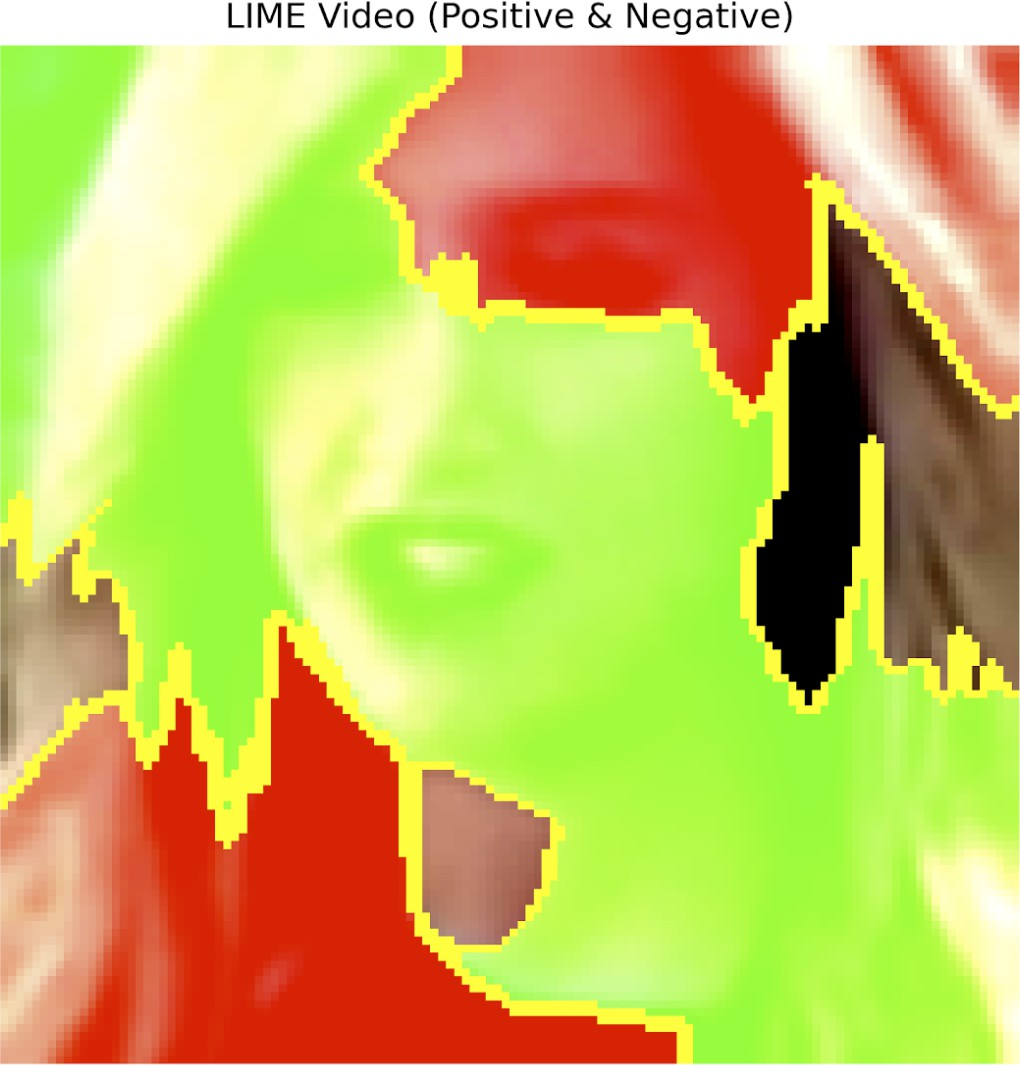
\includegraphics[width=\textwidth]{images/image6.jpeg}
\caption{Full Model}
\end{subfigure}\hfill
\begin{subfigure}[b]{0.48\textwidth}
\centering
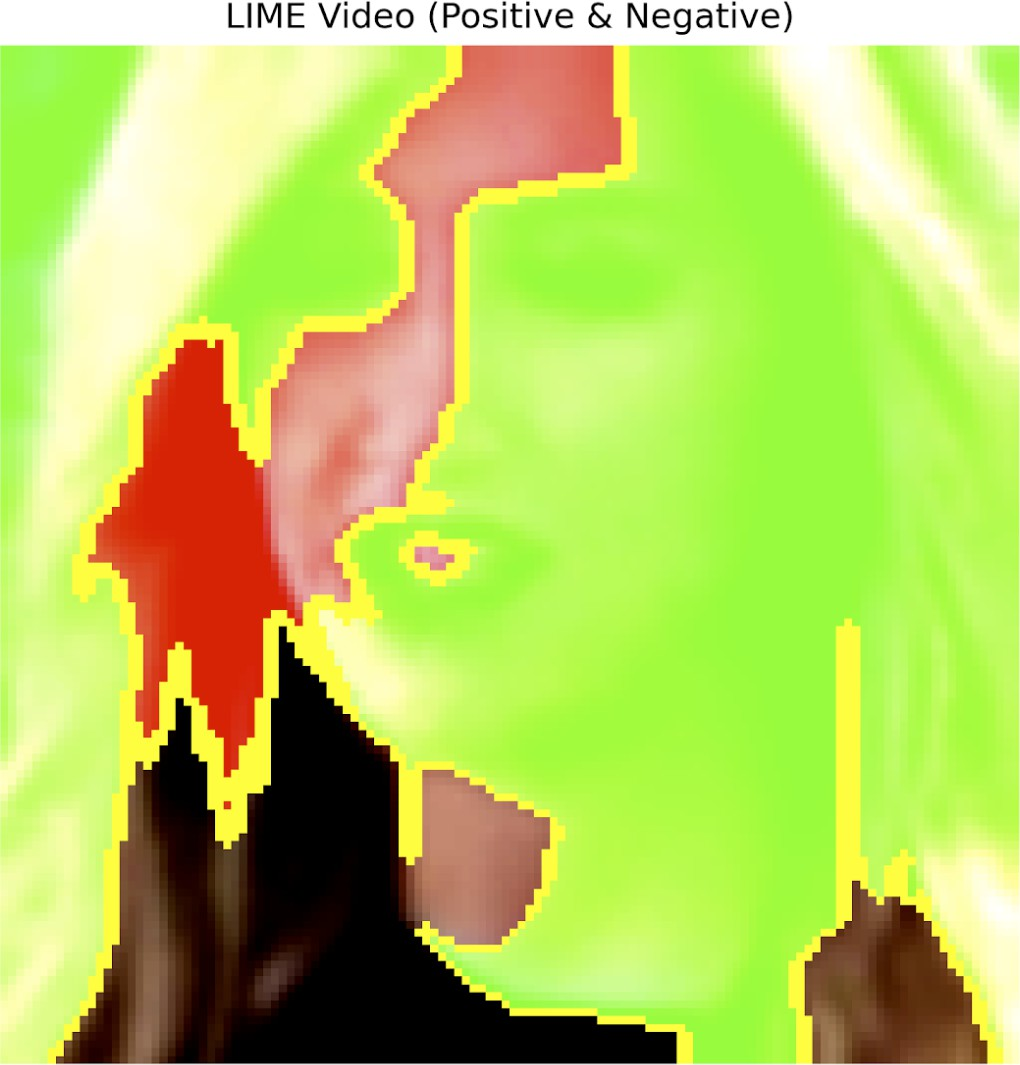
\includegraphics[width=\textwidth]{images/image7.jpeg}
\caption{No-Sync-Loss}
\end{subfigure}\\[6pt]
\begin{subfigure}[b]{0.48\textwidth}
\centering
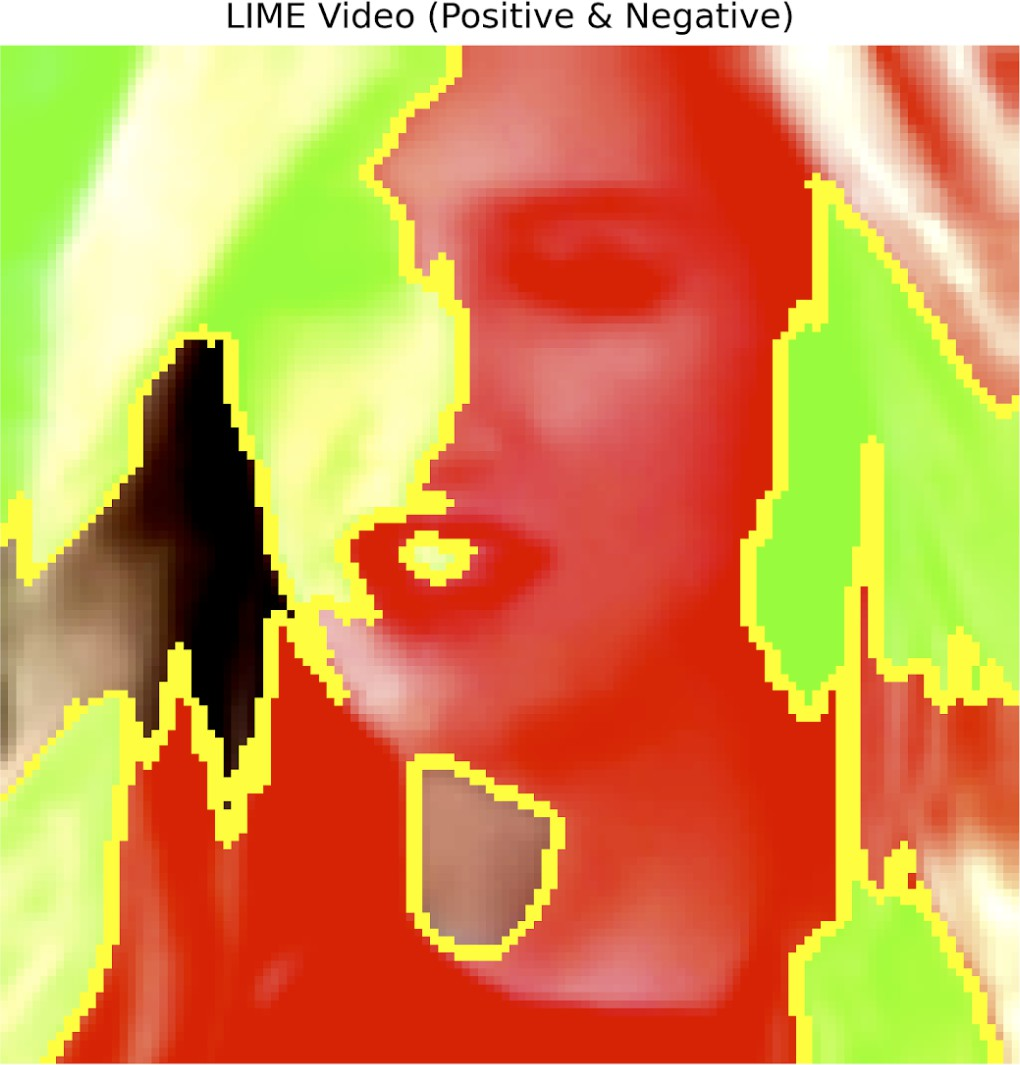
\includegraphics[width=\textwidth]{images/image8.jpeg}
\caption{No-Gate}
\end{subfigure}\hfill
\begin{subfigure}[b]{0.48\textwidth}
\centering
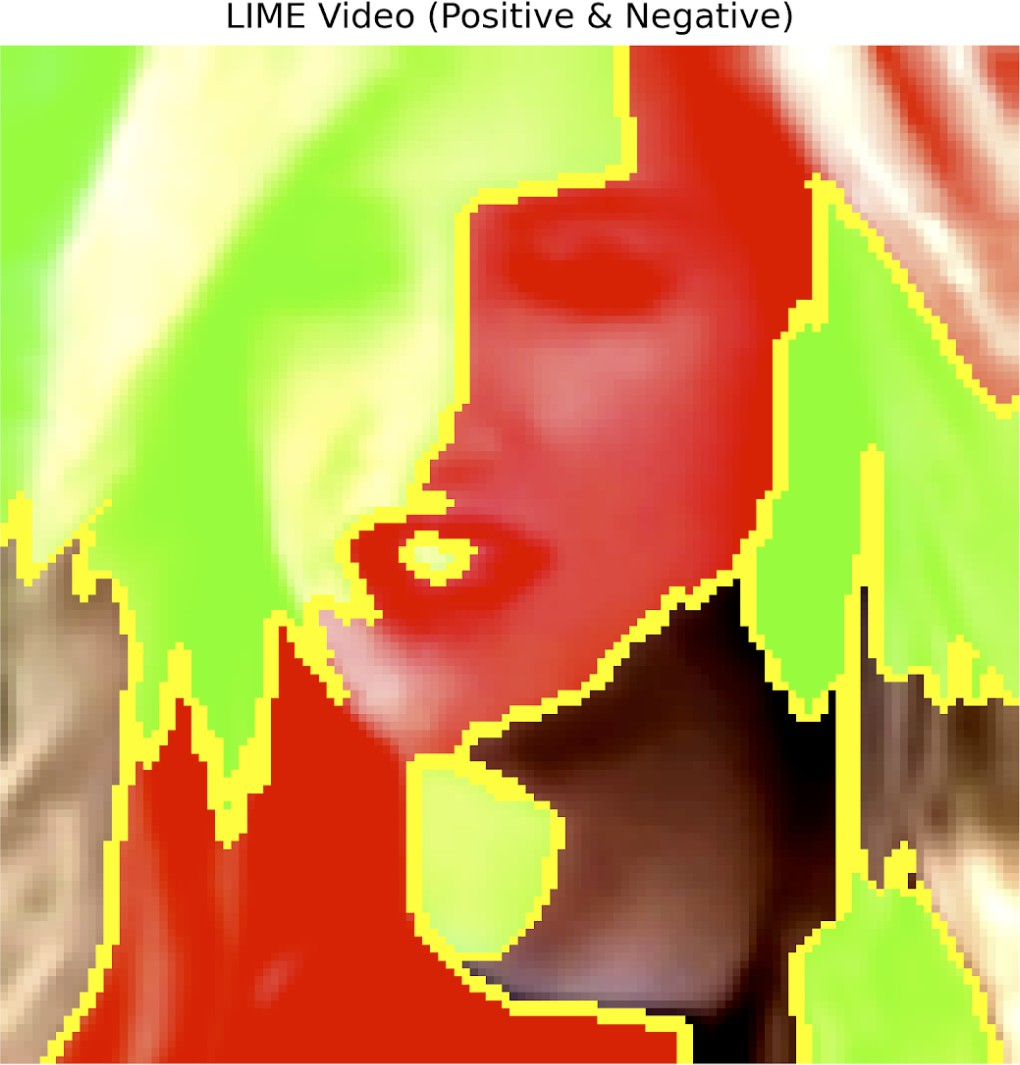
\includegraphics[width=\textwidth]{images/image9.jpeg}
\caption{No-Curriculum}
\end{subfigure}
\caption{LIME visualizations across model variants. The full model concentrates on the mouth region, while ablated variants produce more diffuse or less stable heatmaps.}\label{fig4}
\end{figure}

The qualitative explanations follow the same pattern as the ablation metrics. Figure~\ref{fig4} shows that the full model concentrates evidence near the mouth region, while ablated variants produce less coherent saliency. This supports the interpretation that the removed components affect both accuracy and explanation quality.

Table~\ref{tab6} reports quantitative explanation metrics for the full model and ablations. PinPoint produces moderate video sparsity (Gini 0.631), very concentrated audio attribution (Gini 0.928), and the highest inter-technique consistency among the evaluated variants (Spearman 0.514). Higher Gini values in the ablations should not be interpreted as automatically better: a sparse map can still be unstable or concentrated on spurious evidence. The consistency metric therefore complements the sparsity measure by testing whether different explanation methods agree.
\begin{table}[htbp]
\caption{Quantitative XAI Metrics Across Model Variants}\label{tab6}
\begin{tabular*}{\textwidth}{@{\extracolsep\fill}lccc@{}}
\toprule
\textbf{Model} & \textbf{Video Gini} & \textbf{Audio Gini} & \textbf{Consistency (Spearman)} \\
\midrule
PinPoint (Full, Ours) & 0.631 & 0.928 & 0.514 \\
No-Curriculum & 0.803 & 0.919 & 0.450 \\
No-Gate & 0.753 & 0.760 & 0.372 \\
No-Sync-Loss & 0.708 & 0.883 & 0.436 \\
\midrule
Baldassarre et al. \cite{ref4} & 0.45--0.68 & --- & --- \\
\botrule
\end{tabular*}
\end{table}


\subsection{XAI-Driven Model Interpretation and Case Studies}\label{sec5.3}

The following case studies illustrate how the XAI suite connects PinPoint's predictions to interpretable forensic cues.

\begin{figure}[H]
\centering
\begin{subfigure}[b]{0.48\textwidth}
\centering
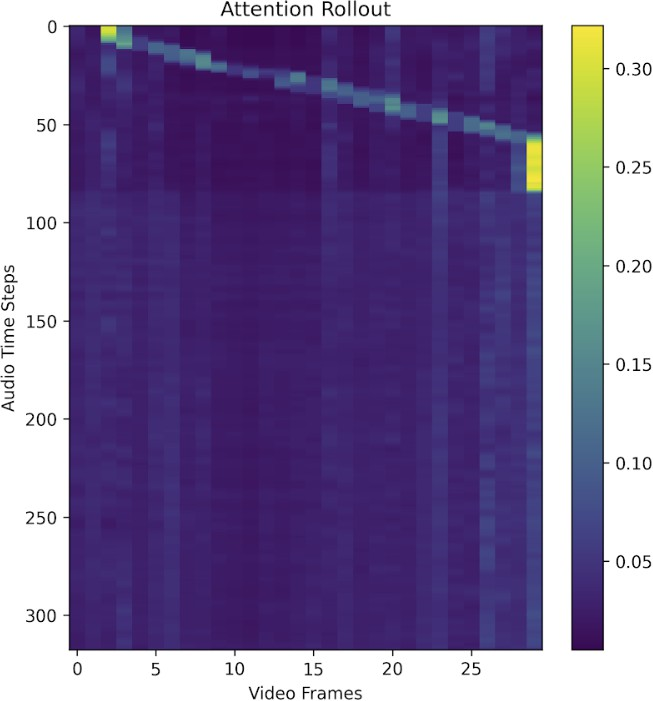
\includegraphics[width=0.6\textwidth]{images/image10.jpeg}
\caption{Real sample (diagonal)}
\end{subfigure}\hfill
\begin{subfigure}[b]{0.48\textwidth}
\centering
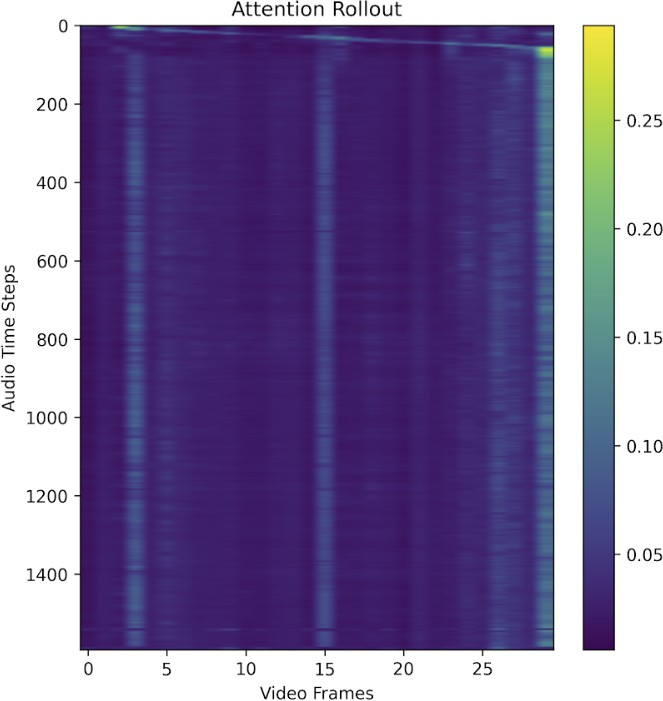
\includegraphics[width=0.6\textwidth]{images/image11.jpeg}
\caption{Fake sample (diffuse)}
\end{subfigure}
\caption{Cross-attention maps. Real samples show stronger diagonal alignment, while fake samples exhibit diffuse attention, indicating weaker audio--visual synchrony.}\label{fig5}
\end{figure}

\textbf{Case Study 1: Pinpointing synchronization breaks.} Figure~\ref{fig5} compares cross-attention maps for real and fake samples. Real samples exhibit stronger diagonal structure, reflecting correspondence between speech acoustics and facial motion. Fake samples show diffuse attention, which indicates that the model has learned desynchronization as a discriminative cue.

\begin{figure}[H]
\centering
\begin{subfigure}[b]{0.32\textwidth}
\centering
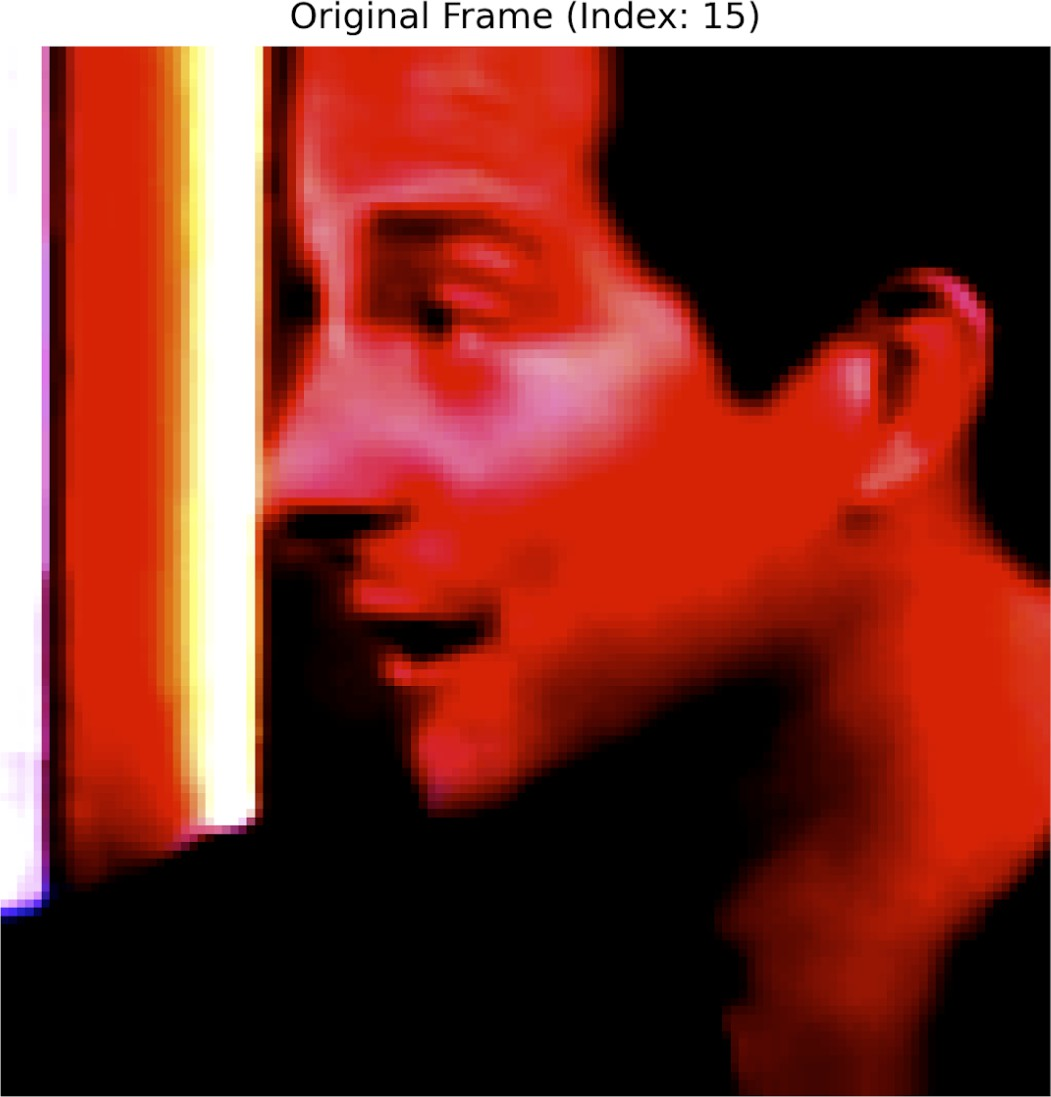
\includegraphics[width=\textwidth]{images/image12.jpeg}
\caption{Original Frame}
\end{subfigure}\hfill
\begin{subfigure}[b]{0.32\textwidth}
\centering
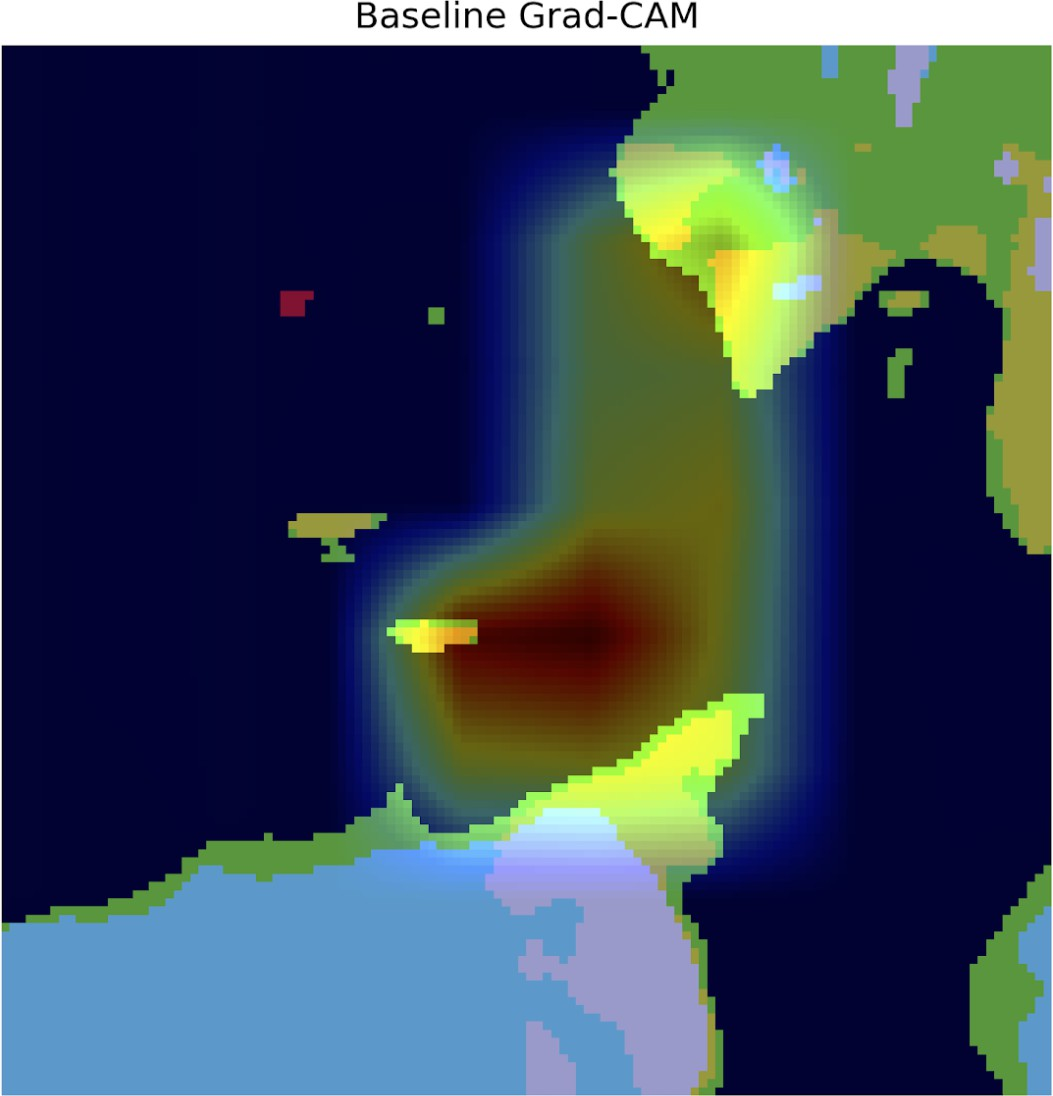
\includegraphics[width=\textwidth]{images/image13.jpeg}
\caption{Baseline Grad-CAM}
\end{subfigure}\hfill
\begin{subfigure}[b]{0.32\textwidth}
\centering
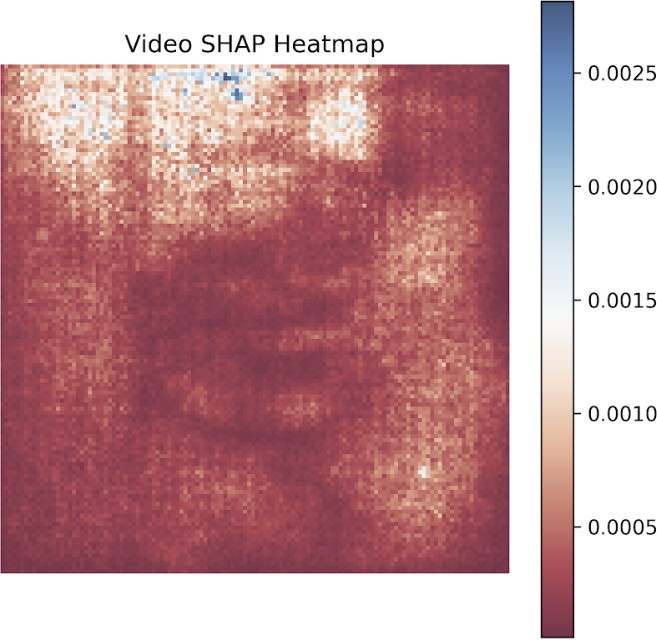
\includegraphics[width=\textwidth]{images/image14.jpeg}
\caption{Video SHAP Heatmap}
\end{subfigure}
\caption{Multimodal attribution. Grad-CAM highlights mouth-region evidence, while SHAP identifies acoustic-feature contributions that complement the visual signal.}\label{fig6}
\end{figure}

\textbf{Case Study 2: Deconstructing subtle multimodal forgeries.} Figure~\ref{fig6} shows a case where visual evidence around the mouth and acoustic evidence in the MFCC sequence jointly support the fake prediction. This case demonstrates that neither the visual nor the acoustic evidence alone would support a confident fake prediction; the gated cross-attention fusion combines both weak signals into a confident classification, and joint attribution maps confirm that neither stream is ignored.

\begin{figure}[H]
\centering
\begin{subfigure}[b]{0.32\textwidth}
\centering
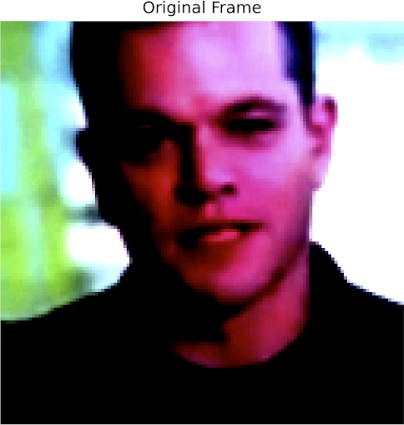
\includegraphics[width=\textwidth]{images/image16.jpeg}
\caption{Original Frame}
\end{subfigure}\hfill
\begin{subfigure}[b]{0.32\textwidth}
\centering
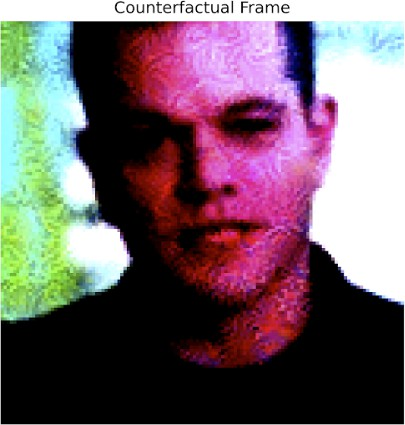
\includegraphics[width=\textwidth]{images/image17.jpeg}
\caption{Counterfactual Frame}
\end{subfigure}\hfill
\begin{subfigure}[b]{0.32\textwidth}
\centering
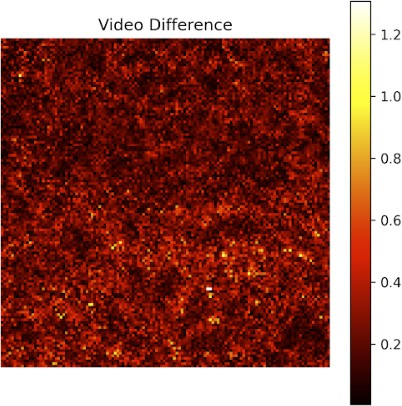
\includegraphics[width=\textwidth]{images/image15.jpeg}
\caption{Video Difference}
\end{subfigure}
\caption{Counterfactual explanation. A small perturbation changes the model decision from fake to real, and the difference map localizes the visual evidence most responsible for the decision flip.}\label{fig7}
\end{figure}

\textbf{Case Study 3: Causal validation via counterfactuals.} Figure~\ref{fig7} shows a counterfactual perturbation that changes a fake prediction to real. The perturbation map indicates which visual changes most influenced the decision boundary. This analysis complements attribution maps because it tests whether modifying the highlighted evidence can actually change the prediction.

\begin{figure}[H]
\centering
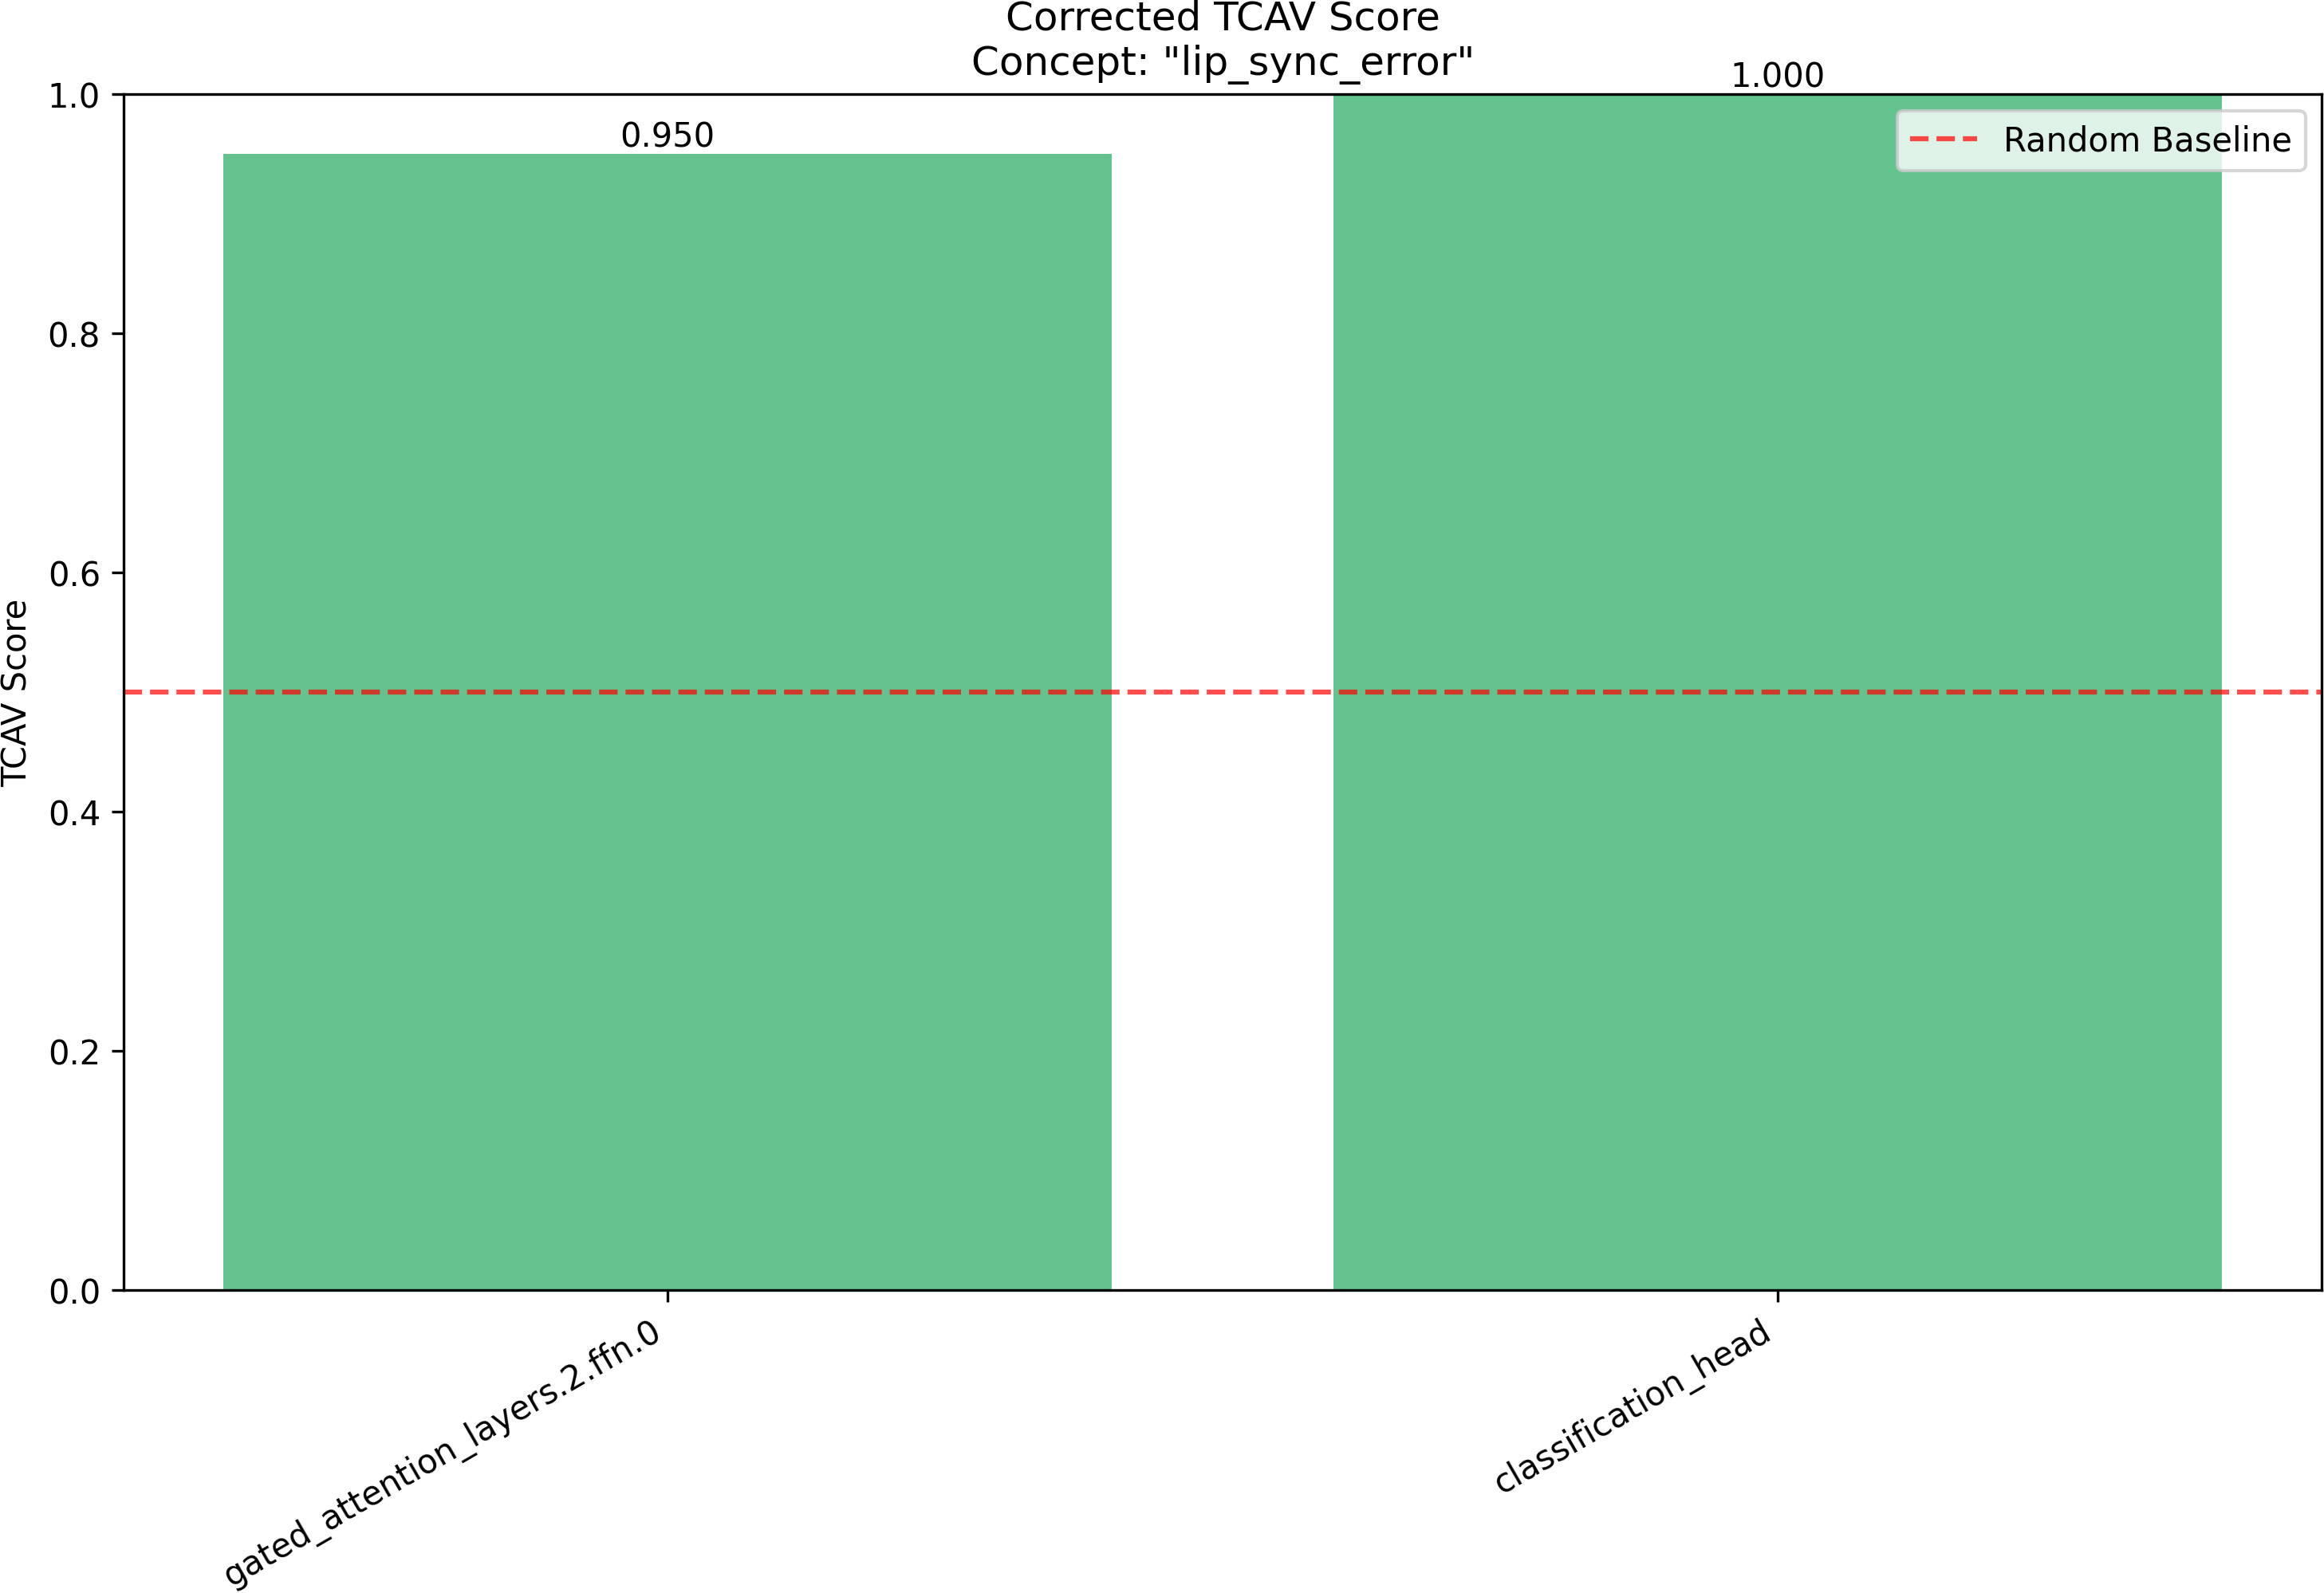
\includegraphics[width=0.7\textwidth]{images/image18.png}
\caption{TCAV scores for the lip-sync error concept. The model shows high concept sensitivity at the gated attention layer and classification head, indicating that synchronization cues influence the learned representation.}\label{fig8}
\end{figure}

\textbf{Case Study 4: Validating concept learning with TCAV.} Figure~\ref{fig8} evaluates sensitivity to the lip-sync error concept. The model reaches a TCAV score of 0.950 at the gated attention layer and 1.000 at the classification head, both above the random baseline of 0.5. These scores indicate that synchronization-related concepts influence the internal representation and final decision.


\section{Discussion}\label{sec6}

The results support the central design claim of PinPoint: when temporal synchrony is supervised directly, the detector becomes both more accurate and easier to inspect. The ablation study shows that synchronization loss, gated fusion, and curriculum training all contribute to performance, while the XAI analysis shows that the full model produces more consistent explanations than the weaker variants. This matters for forensic use because an examiner needs more than a binary label; the system should expose the visual, acoustic, and temporal evidence behind that label.

PinPoint also narrows the gap between optimization and explanation. Instead of applying XAI only after training, the synchronization loss makes diagonal attention an expected property of real aligned samples. The attention maps therefore have a task-specific interpretation, and the other XAI tools can be used to check whether the model's local attributions, counterfactuals, and concept activations agree with that interpretation.


\subsection{Limitations and Future Work}\label{sec6.1}

\textbf{Computational cost.} The full XAI suite is expensive because SHAP, counterfactual generation, and attribution methods require additional forward or backward passes. A lighter deployment version may need distillation or selective explanation modes.

\textbf{In-the-wild robustness.} The current evaluation uses curated benchmark data. Future work should test videos from uncontrolled social-media, messaging, and compressed streaming environments.

\textbf{Temporal scope.} The model uses fixed 30-frame segments. Longer-range inconsistencies may require hierarchical temporal modeling or sliding-window aggregation.

\textbf{Unknown manipulations.} PinPoint remains a supervised detector. Open-set or unsupervised extensions are needed to identify manipulation families that are not represented during training.

\textbf{Cross-dataset generalization.} The unified benchmark mixes LAV-DF and FakeAVCeleb, but a stricter protocol should train on one dataset and test on another to measure transfer under stronger distribution shift.


\section{Conclusion}

This paper presented PinPoint, a synchronization-aware audio--visual deepfake detector designed for both classification performance and forensic inspection. The model combines a ResNet-18 video encoder, a CNN--GRU audio encoder, gated cross-attention, curriculum learning, and a multi-component synchronization loss that shapes attention maps toward temporally meaningful structure.

Taken together, these results suggest that synchronization-aware supervision is structural rather than merely additive. The largest accuracy drops occur when components that directly enforce temporal correspondence are removed, while the curriculum result shows that training order shapes the cues the model learns to rely on. The XAI analysis supports the same conclusion: the full model not only predicts more accurately, but also produces explanations that remain more consistent with synchronization-related evidence than those of the ablated variants.

The main lesson is that interpretability should not be treated only as a post-hoc add-on for deepfake detection. By making synchronization part of the training objective and then auditing the resulting model with attribution, attention, counterfactual, and concept-based tools, PinPoint provides a more transparent path toward forensic multimedia analysis. Future work should test the method under stronger cross-dataset and in-the-wild protocols and reduce the cost of the full explanation pipeline.


%%% Mandatory Declaration Sections for Springer NCA %%%
\section{Declarations}

\textbf{Availability of data and material}
The datasets analyzed during the current study (LAV-DF and FakeAVCeleb) are publicly available in their
respective official repositories. Derived data supporting the findings of this study are available from the corresponding author upon reasonable request.\newline
\textbf{Competing interests} 
The authors declare that they have no known competing financial interests or personal relationships that could have appeared to influence the work reported in this paper. \newline
\textbf{Funding}
This research did not receive any specific grant from funding agencies in the public, commercial, or not-for-profit sectors. \newline
\textbf{Authors' contributions}
Palak Parmar and Chintan Bhatt wrote the main manuscript text, and SantoshKumar Bharti prepared Figures 1--3. All authors reviewed the manuscript. \newline
\textbf{Acknowledgements} 
The authors would like to acknowledge the open-source community for the foundational tools and datasets
that enabled this research.

\backmatter





\begin{thebibliography}{24}

\bibitem{ref1}
Raza, M.A., Malik, K.M.: Multimodaltrace: Deepfake Detection using Audiovisual Representation Learning. In: Proceedings of the IEEE/CVF Conference on Computer Vision and Pattern Recognition (CVPR) Workshops (2023). \url{https://doi.org/10.1109/CVPRW59228.2023.00048}

\bibitem{ref2}
Gao, Y., Wang, X., Zhang, Y., Zeng, P., Ma, Y.: Temporal Feature Prediction in Audio-Visual Deepfake Detection. Electronics \textbf{13}(1) (2024). \url{https://doi.org/10.3390/electronics13010095}

\bibitem{ref3}
Xu, Y., Raja, K., Pedersen, M.: Supervised Contrastive Learning for Generalizable and Explainable DeepFakes Detection. In: Proceedings of the IEEE/CVF Winter Conference on Applications of Computer Vision (WACV) Workshops (2022). \url{https://doi.org/10.1109/WACVW54805.2022.00039}

\bibitem{ref4}
Baldassarre, F., Debard, Q., Pontiveros, G.F., Wijaya, T.K.: Quantitative Metrics for Evaluating Explanations of Video DeepFake Detectors. arXiv preprint arXiv:2210.01353 (2022). \url{https://doi.org/10.48550/arXiv.2210.01353}

\bibitem{ref5}
Javed, M., et al.: Audio-Visual Synchronization and Lip Movement Analysis for Real-Time Deepfake Detection. Int. J. Comput. Intell. Syst. (2025). \url{https://doi.org/10.1007/s44196-025-00755-z}

\bibitem{ref6}
Raval, H.H., Patel, M.S., Parmar, S.D.: A Review on Explainable AI for Deepfake Detection Leveraging Hybrid Deep Learning Techniques. SPU-J. Sci. Technol. Manag. Res. (SPU-JSTMR) (2025)

\bibitem{ref7}
Du, Y., et al.: CAD: A General Multimodal Framework for Video Deepfake Detection via Cross-Modal Alignment and Distillation. arXiv preprint arXiv:2501.03829 (2025). \url{https://doi.org/10.48550/arXiv.2501.03829}

\bibitem{ref8}
Tsigos, K., et al.: Towards Quantitative Evaluation of Explainable AI Methods for Deepfake Detection. In: Proceedings of the 3rd ACM International Workshop on Multimedia AI against Disinformation (MAD '24) (2024). \url{https://doi.org/10.1145/3643491.3660291}

\bibitem{ref9}
Hondru, V., Hogea, E., Onchis, D., Ionescu, R.T.: ExDDV: A New Dataset for Explainable Deepfake Detection in Video. arXiv preprint arXiv:2501.07632 (2025). \url{https://doi.org/10.48550/arXiv.2501.07632}

\bibitem{ref10}
Yu, C., et al.: Explicit Correlation Learning for Generalizable Cross-Modal Deepfake Detection. arXiv preprint arXiv:2403.11183 (2024). \url{https://doi.org/10.48550/arXiv.2403.11183}

\bibitem{ref11}
Koutlis, C., Papadopoulos, S.: DiMoDif: Discourse Modality-information Differentiation for Audio-visual Deepfake Detection and Localization. arXiv preprint arXiv:2403.04273 (2024). \url{https://doi.org/10.48550/arXiv.2403.04273}

\bibitem{ref12}
Wu, X., et al.: HOLA: Enhancing Audio-visual Deepfake Detection via Hierarchical Contextual Aggregations and Efficient Pre-training. In: Proceedings of the ACM International Conference on Multimedia (MM '25) (2025). \url{https://doi.org/10.1145/3664647.3681534}

\bibitem{ref13}
Hashmi, A., et al.: Understanding Audiovisual Deepfake Detection: Techniques, Challenges, Human Factors and Perceptual Insights. arXiv preprint arXiv:2404.03260 (2024). \url{https://doi.org/10.48550/arXiv.2404.03260}

\bibitem{ref14}
Tariq, S., et al.: From Prediction to Explanation: Multimodal, Explainable, and Interactive Deepfake Detection Framework for Non-Expert Users. In: Proceedings of the ACM International Conference on Multimedia (MM '25) (2025). \url{https://doi.org/10.1145/3664647.3685629}

\bibitem{ref15}
Karne, S., et al.: Enhancing Deepfake Detection with Explainable AI. In: Proceedings of the 3rd International Conference on Networking, Multimedia and Information Technology (NMITCON) (2025). \url{https://doi.org/10.1109/NMITCON62075.2025.10823574}

\bibitem{ref16}
Croitoru, F.-A., et al.: MAVOS-DD: Multilingual Audio-Video Open-Set Deepfake Detection Benchmark. arXiv preprint arXiv:2503.06456 (2025). \url{https://doi.org/10.48550/arXiv.2503.06456}

\bibitem{ref17}
Alotaibi, S.: Revealing the Unseen: An Insightful Survey on Explainable AI for Deepfake Face Detection. In: Proceedings of the 17th International Conference on Developments in eSystems Engineering (DeSE) (2024). \url{https://doi.org/10.1109/DeSE62575.2024.10798975}

\bibitem{ref18}
Ilyas, H., Javed, A., Malik, K.M.: ConvNext-PNet: An interpretable and explainable deep-learning model for deepfakes detection. In: Proceedings of the IEEE International Joint Conference on Biometrics (IJCB) (2024). \url{https://doi.org/10.1109/IJCB62174.2024.10744521}

\bibitem{ref19}
Chen, Y., et al.: x\textsuperscript{2}-DFD: A framework for explainable and extendable Deepfake Detection. arXiv preprint (2025). \url{https://doi.org/10.48550/arXiv.2504.07109}

\bibitem{ref20}
Rahman, T., Chakma, R., Mahmud, T.: Beyond Accuracy: Explainable Multimodal Deepfake Detection Through Cross-Modal Feature Analysis and Dynamic Attention Weighting. In: Proceedings of the International Conference on Quantum, Photonics, Artificial Intelligence and Networking (QPAIN) (2025). \url{https://doi.org/10.1109/QPAIN64062.2025.10810756}

\bibitem{ref21}
Malolan, B., Parekh, A., Kazi, F.: Explainable Deep-Fake Detection Using Visual Interpretability Methods. In: Proceedings of the 3rd International Conference on Information and Computer Technologies (ICICT), pp.~103--108 (2020). \url{https://doi.org/10.1109/ICICT50521.2020.00024}

\bibitem{ref22}
Nguyen-Le, H.-H., Tran, V.-T., Nguyen, D.-T., Le-Khac, N.-A.: Passive Deepfake Detection: A Comprehensive Survey across Multi-modalities. arXiv preprint (2025). \url{https://doi.org/10.48550/arXiv.2502.04818}

\bibitem{ref23}
Kundu, R., et al.: TruthLens: Visual Grounding for Universal DeepFake Reasoning. arXiv preprint (2025). \url{https://doi.org/10.48550/arXiv.2503.14148}

\bibitem{ref24}
Khalid, F., Javed, A., Malik, K.M., Irtaza, A.: ExplaNET: A Descriptive Framework for Detecting Deepfakes With Interpretable Prototypes. IEEE Trans. Biom. Behav. Identity Sci. (2024). \url{https://doi.org/10.1109/TBIOM.2024.3462874}

\end{thebibliography}

\end{document}
